\section{Results}\label{sec:results}

We organized our experimental evaluation into four parts: (1) analysis of the 2DPCA eigenvalue spectrum and spatial reconstruction residuals; (2) cross-validation across stratified, temporally grouped, and FOV-masked splits; (3) baseline and ablation comparisons, including zero-shot transfer to an unseen observatory; and (4) operational evaluation under bright lunar glare, continuous nocturnal monitoring with Stage~1 cloud screening, and pixel-level SHAP attribution.

\subsection{2DPCA Eigenvalue Spectrum and Reconstruction Residuals}

To select the number of 2DPCA projection vectors $k$ objectively, we inspected the full 64-component eigenvalue spectrum of the $64 \times 64$ image covariance matrix together with the 5-fold cross-validated F1-score on the training split across $k \in \{1, 2, 3, 5, 10, 15, 20, 25, 30\}$ (Figure~\ref{fig:2dpca_variance}).

\begin{figure}[htbp]
    \centering
    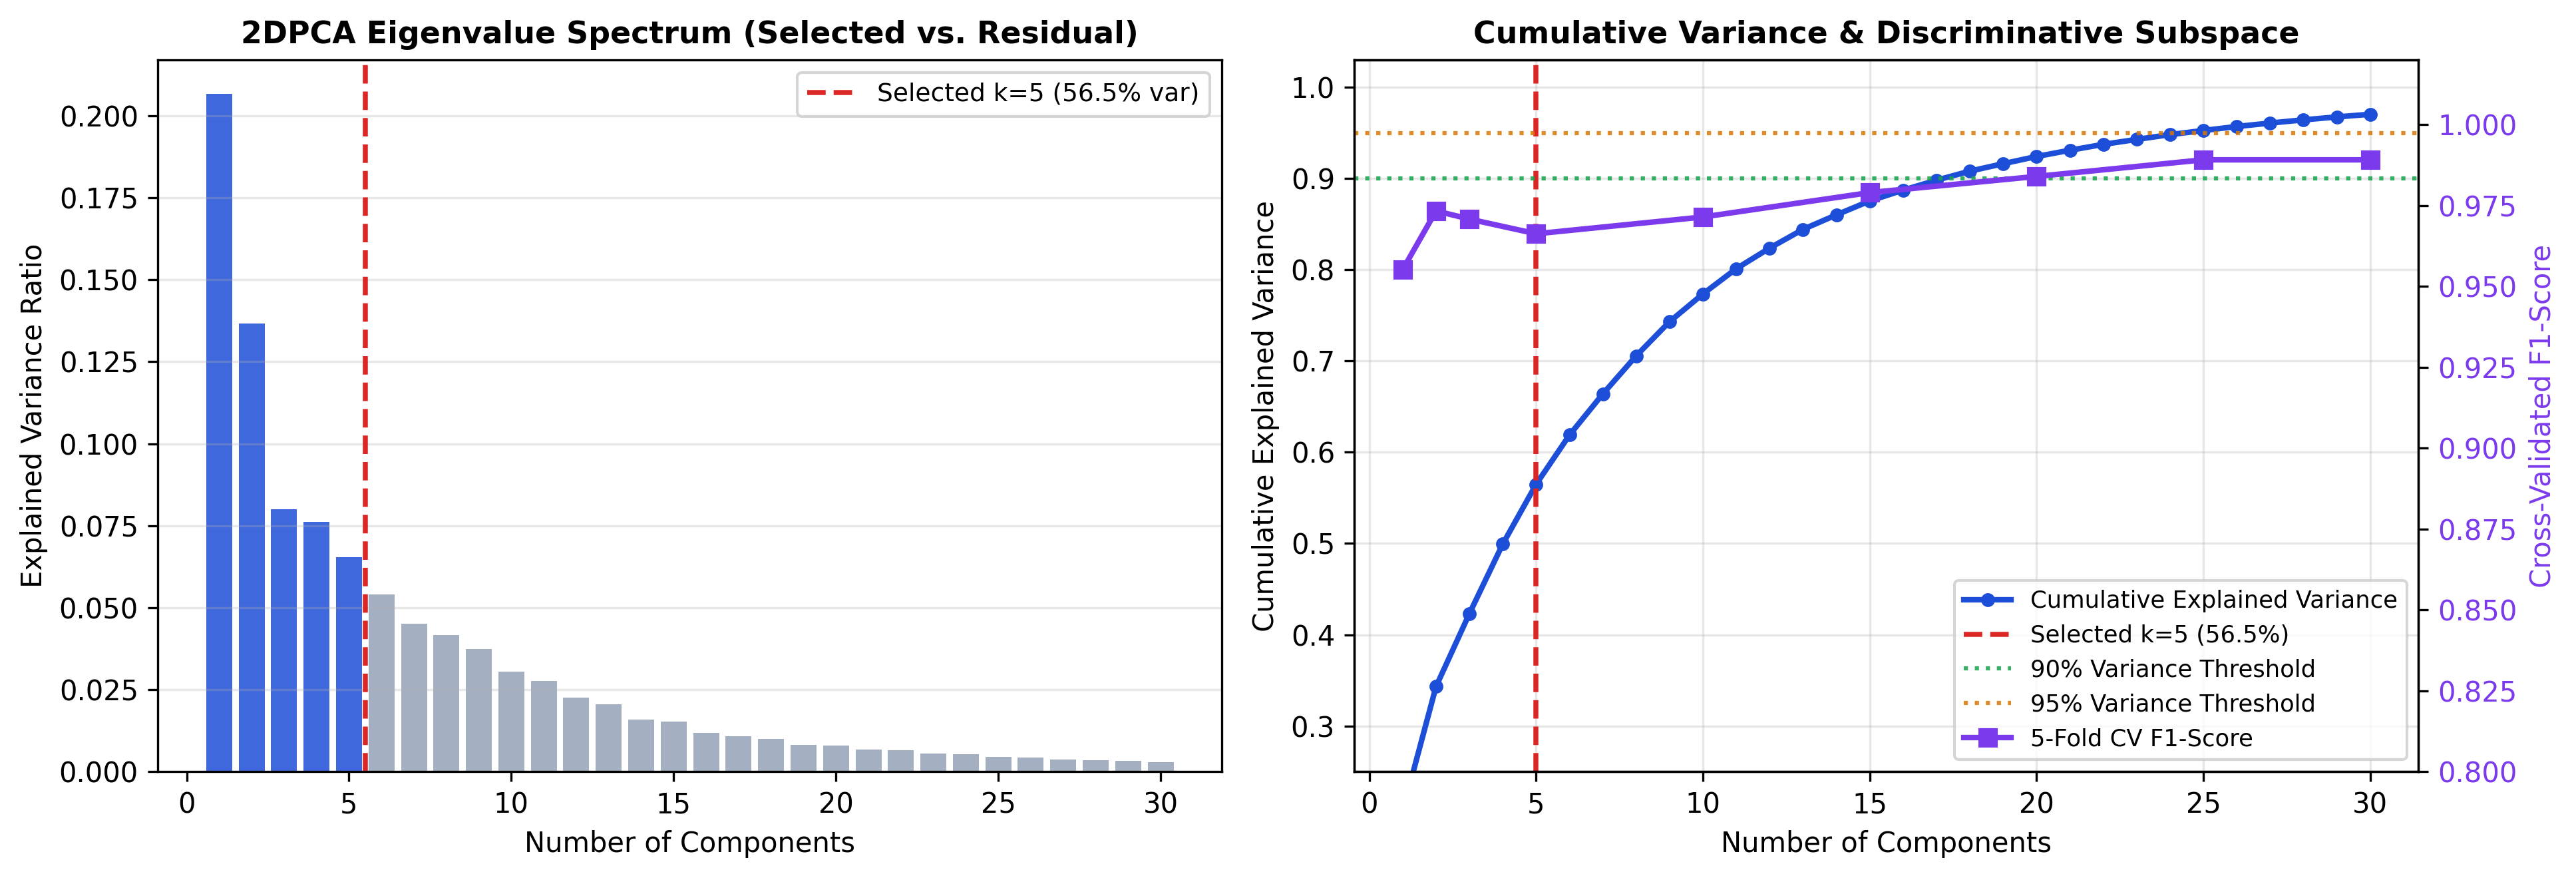
\includegraphics[width=0.98\textwidth]{figs/2dpca_variance.png}
    \caption{Left: Individual explained variance ratio across the first $30$ 2DPCA components (out of $64$) on the augmented training split, indicating the selected $k=5$ cutoff ($56.5\%$ cumulative variance). Right: Cumulative explained variance and 5-fold cross-validated F1-score from $k=1$ to $k=30$.}
    \label{fig:2dpca_variance}
\end{figure}

Because Stage~2 subtracts the smooth Gaussian dome background ($\sigma=10$) and equalizes local contrast via CLAHE prior to covariance estimation, the dominant uniform illumination mode (which accounts for nearly $80\%$ of raw image variance) is already removed. Consequently, spatial variance is distributed across a broader set of eigenvectors: on the unaugmented training set ($n=429$), cumulative variance rises from $22.86\%$ ($k=1$) and $46.27\%$ ($k=3$) to $59.41\%$ at $k=5$, $79.03\%$ at $k=10$, and $95.69\%$ at $k=25$ (and $56.49\%$ at $k=5$ on the augmented training split shown in Figure~\ref{fig:2dpca_variance}). Even though components $k > 5$ continue to accumulate high-frequency variance from residual star specks and sensor grain, the cross-validated F1-score already exceeds $0.966$ by $k=5$ ($320$ features). Retaining $k=5$ captures the mesoscale horizontal variations of plasma depletion channels while avoiding the higher feature-to-sample ratio ($1600\text{--}1920$ features at $k=25\text{--}30$) that increases overfitting risk across stations.

\begin{figure}[htbp]
    \centering
    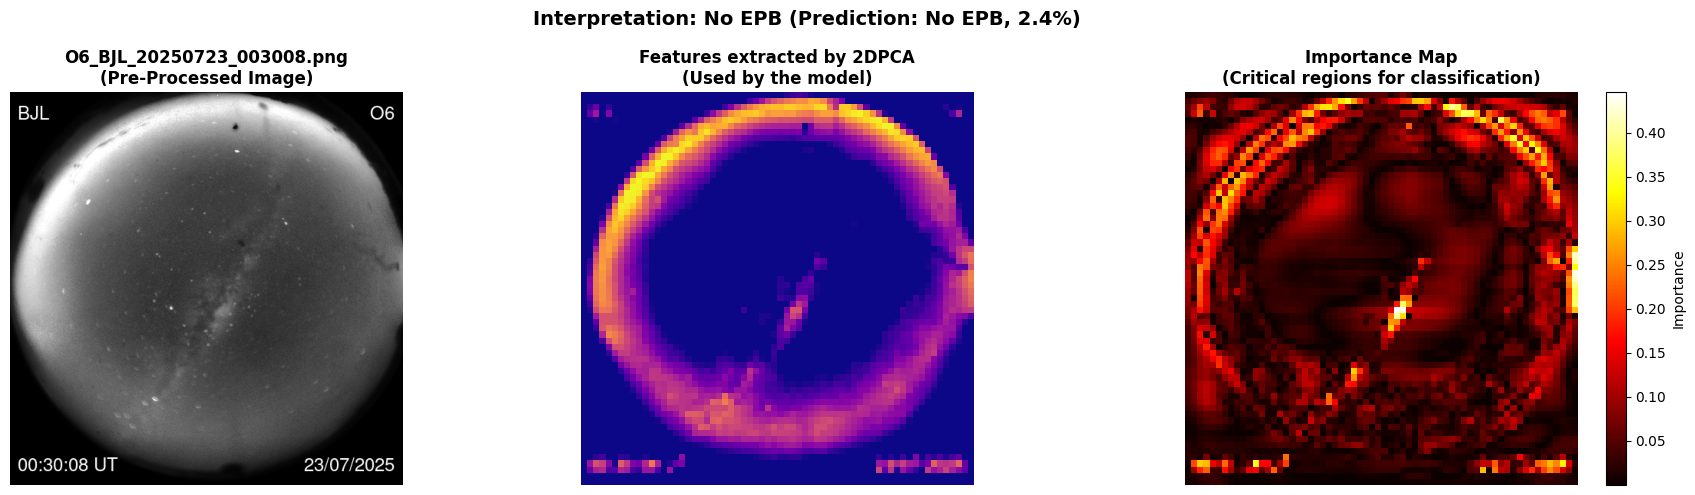
\includegraphics[width=0.96\textwidth]{figs/recon_error_without.png}
    \caption{Unsupervised 2DPCA subspace reconstruction analysis for a quiet-sky exposure (No EPB, predicted EPB probability $0.4\%$). Left: raw $630.0\text{ nm}$ image. Center: preprocessed $64 \times 64$ matrix $\mathbf{X}$. Right: reconstruction residual $|\mathbf{X} - \hat{\mathbf{X}}|$.}
    \label{fig:recon_error_without}
\end{figure}

\begin{figure}[htbp]
    \centering
    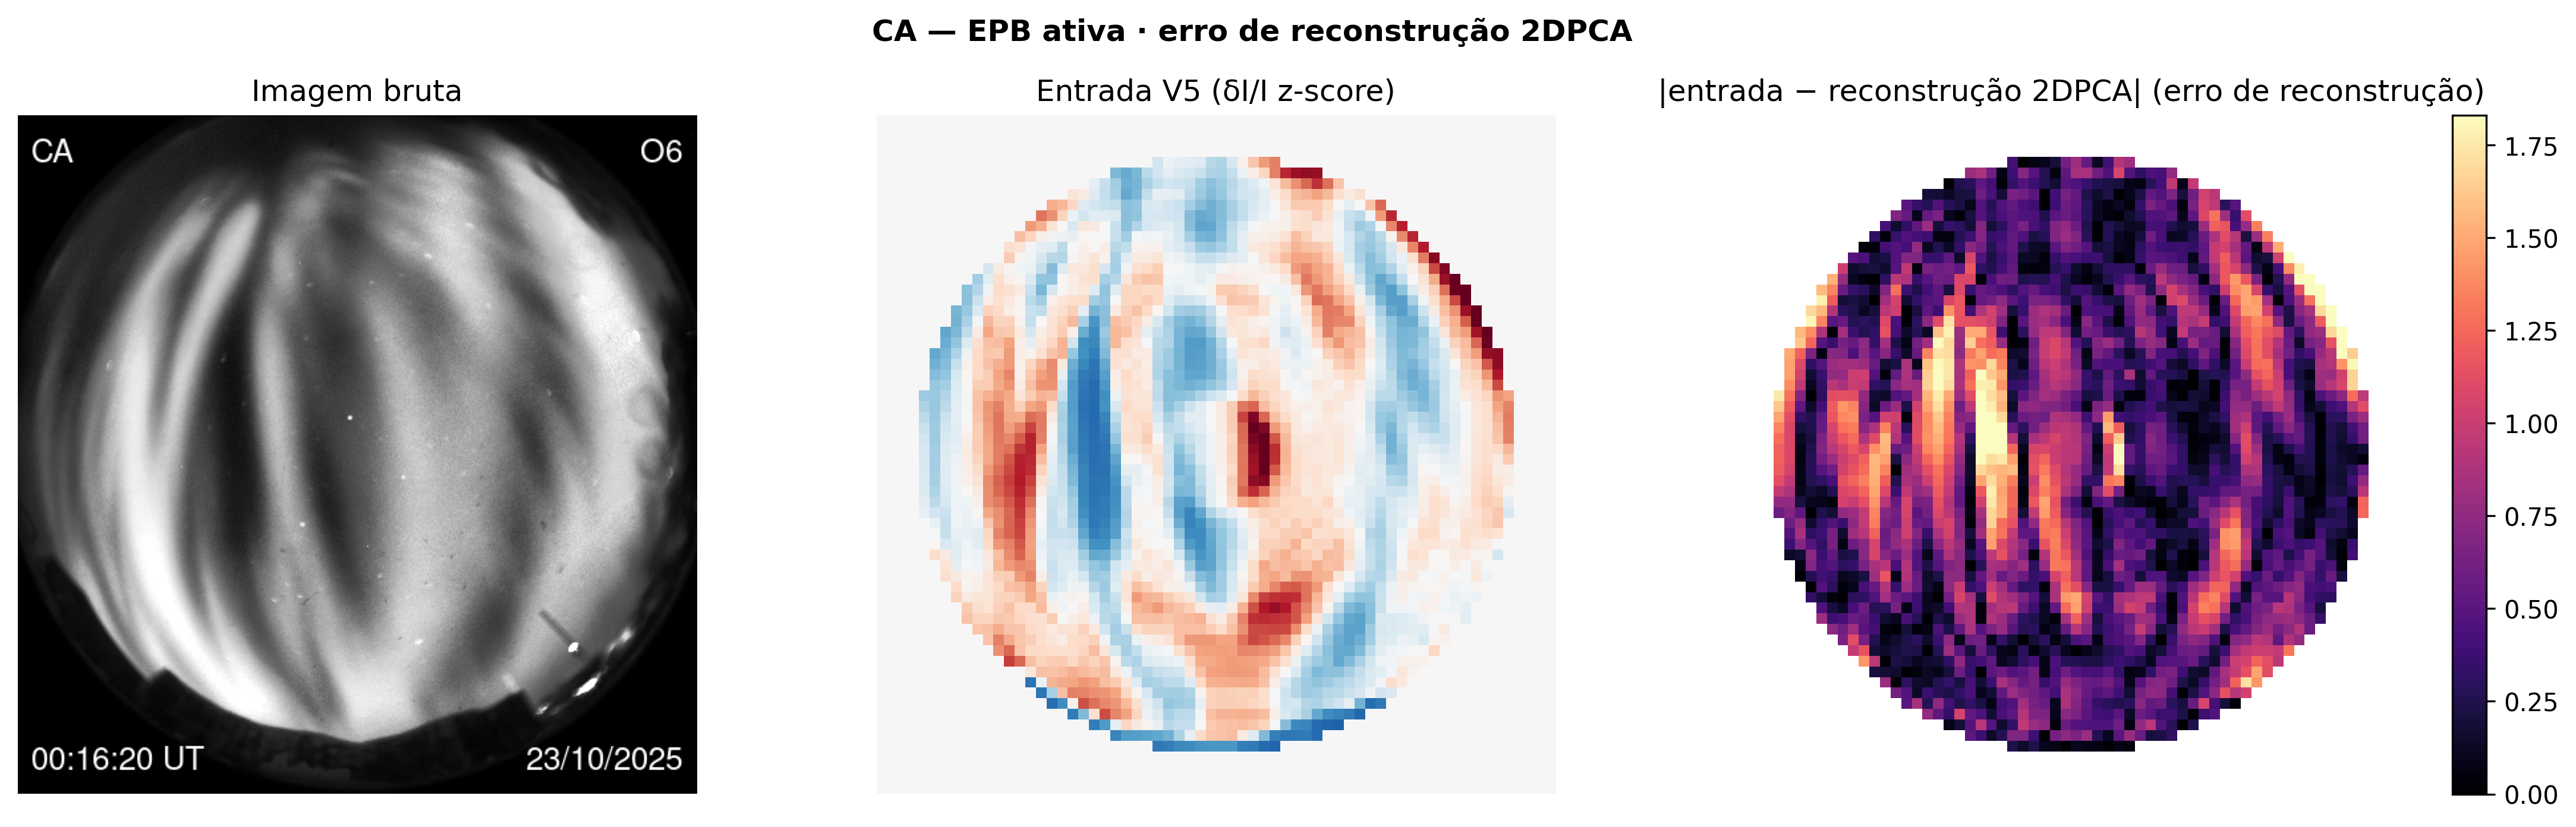
\includegraphics[width=0.96\textwidth]{figs/recon_error_with.png}
    \caption{Unsupervised 2DPCA subspace reconstruction analysis for an active EPB exposure (predicted EPB probability $99.2\%$). Large reconstruction residuals trace the North-South plasma depletion bands.}
    \label{fig:recon_error_with}
\end{figure}

Figures~\ref{fig:recon_error_without} and~\ref{fig:recon_error_with} compare the $k=5$ subspace reconstruction $\hat{\mathbf{X}}$ on quiet and active ionospheric exposures. For the quiet-sky frame from Bom Jesus da Lapa (Figure~\ref{fig:recon_error_without}), the interior of the camera dome shows low reconstruction error, with residuals confined to the outer lens border and a faint central Milky Way streak. For the active EPB frame from Cariri (Figure~\ref{fig:recon_error_with}), the dark, bifurcated plasma depletions introduce steep intensity transitions that produce elevated residuals ($\mathbf{E} > 0.4$) along the entire North-South extent of the bubble channels.

\subsection{Cross-Validation Across Splitting Protocols}

Table~\ref{tab:cv_protocols} reports the classification performance of the 2DPCA ($k=5$) + Stacking Ensemble across our validation protocols on the $N=572$ labeled dataset. Under 5-fold stratified cross-validation (Figure~\ref{fig:kfold_cv}), the model achieves $97.20\% \pm 1.57\%$ accuracy, $95.30\% \pm 4.51\%$ sensitivity, $98.74\% \pm 1.32\%$ specificity, $98.45\% \pm 1.59\%$ precision, $96.78\% \pm 1.86\%$ F1-score, $0.9984 \pm 0.0016$ ROC-AUC, and $0.9980 \pm 0.0018$ PR-AUC. Across all $572$ out-of-fold predictions (Figures~\ref{fig:confusion_matrix} and~\ref{fig:roc_pr}), the ensemble records $313$ true negatives, $4$ false positives, $12$ false negatives, and $243$ true positives (pooled OOF ROC-AUC $= 0.997$, PR-AUC $= 0.996$). On the $25\%$ stratified holdout test set ($n=143$: $64$ EPB and $79$ No-EPB), accuracy is $96.50\%$ ($95.31\%$ sensitivity, $97.47\%$ specificity, $96.83\%$ precision, $96.25\%$ negative predictive value, $96.06\%$ F1-score, and $0.9974$ ROC-AUC).

\begin{table}[htbp]
\centering
\caption{Performance of the 2DPCA ($k=5$) + Stacking Ensemble across validation protocols on the labeled dataset ($N=572$, mean $\pm$ standard deviation across folds).}
\label{tab:cv_protocols}
\resizebox{\textwidth}{!}{%
\setlength{\tabcolsep}{4pt}
\begin{tabular}{lcccccc}
\toprule
\textbf{Validation Protocol} & \textbf{Acc (\%)} & \textbf{Sens (\%)} & \textbf{Spec (\%)} & \textbf{Prec (\%)} & \textbf{F1 (\%)} & \textbf{ROC-AUC} \\
\midrule
5-Fold Stratified CV ($N=572$) & $97.20 \pm 1.57$ & $95.30 \pm 4.51$ & $98.74 \pm 1.32$ & $98.45 \pm 1.59$ & $96.78 \pm 1.86$ & $0.9984 \pm 0.0016$ \\
5-Fold Temporal-Block CV ($77$ blocks) & $95.08 \pm 5.72$ & $90.88 \pm 10.48$ & $98.79 \pm 2.71$ & $98.60 \pm 3.14$ & $94.24 \pm 5.37$ & $0.9969 \pm 0.0066$ \\
5-Fold Circular FOV Mask CV ($N=572$) & $95.80 \pm 1.57$ & $93.34 \pm 4.72$ & $97.79 \pm 1.80$ & $97.24 \pm 2.15$ & $95.16 \pm 1.89$ & $0.9976 \pm 0.0011$ \\
Holdout Test Split ($n=143$) & $96.50$ & $95.31$ & $97.47$ & $96.83$ & $96.06$ & $0.9974$ \\
\bottomrule
\end{tabular}%
}
\end{table}

\begin{figure}[htbp]
    \centering
    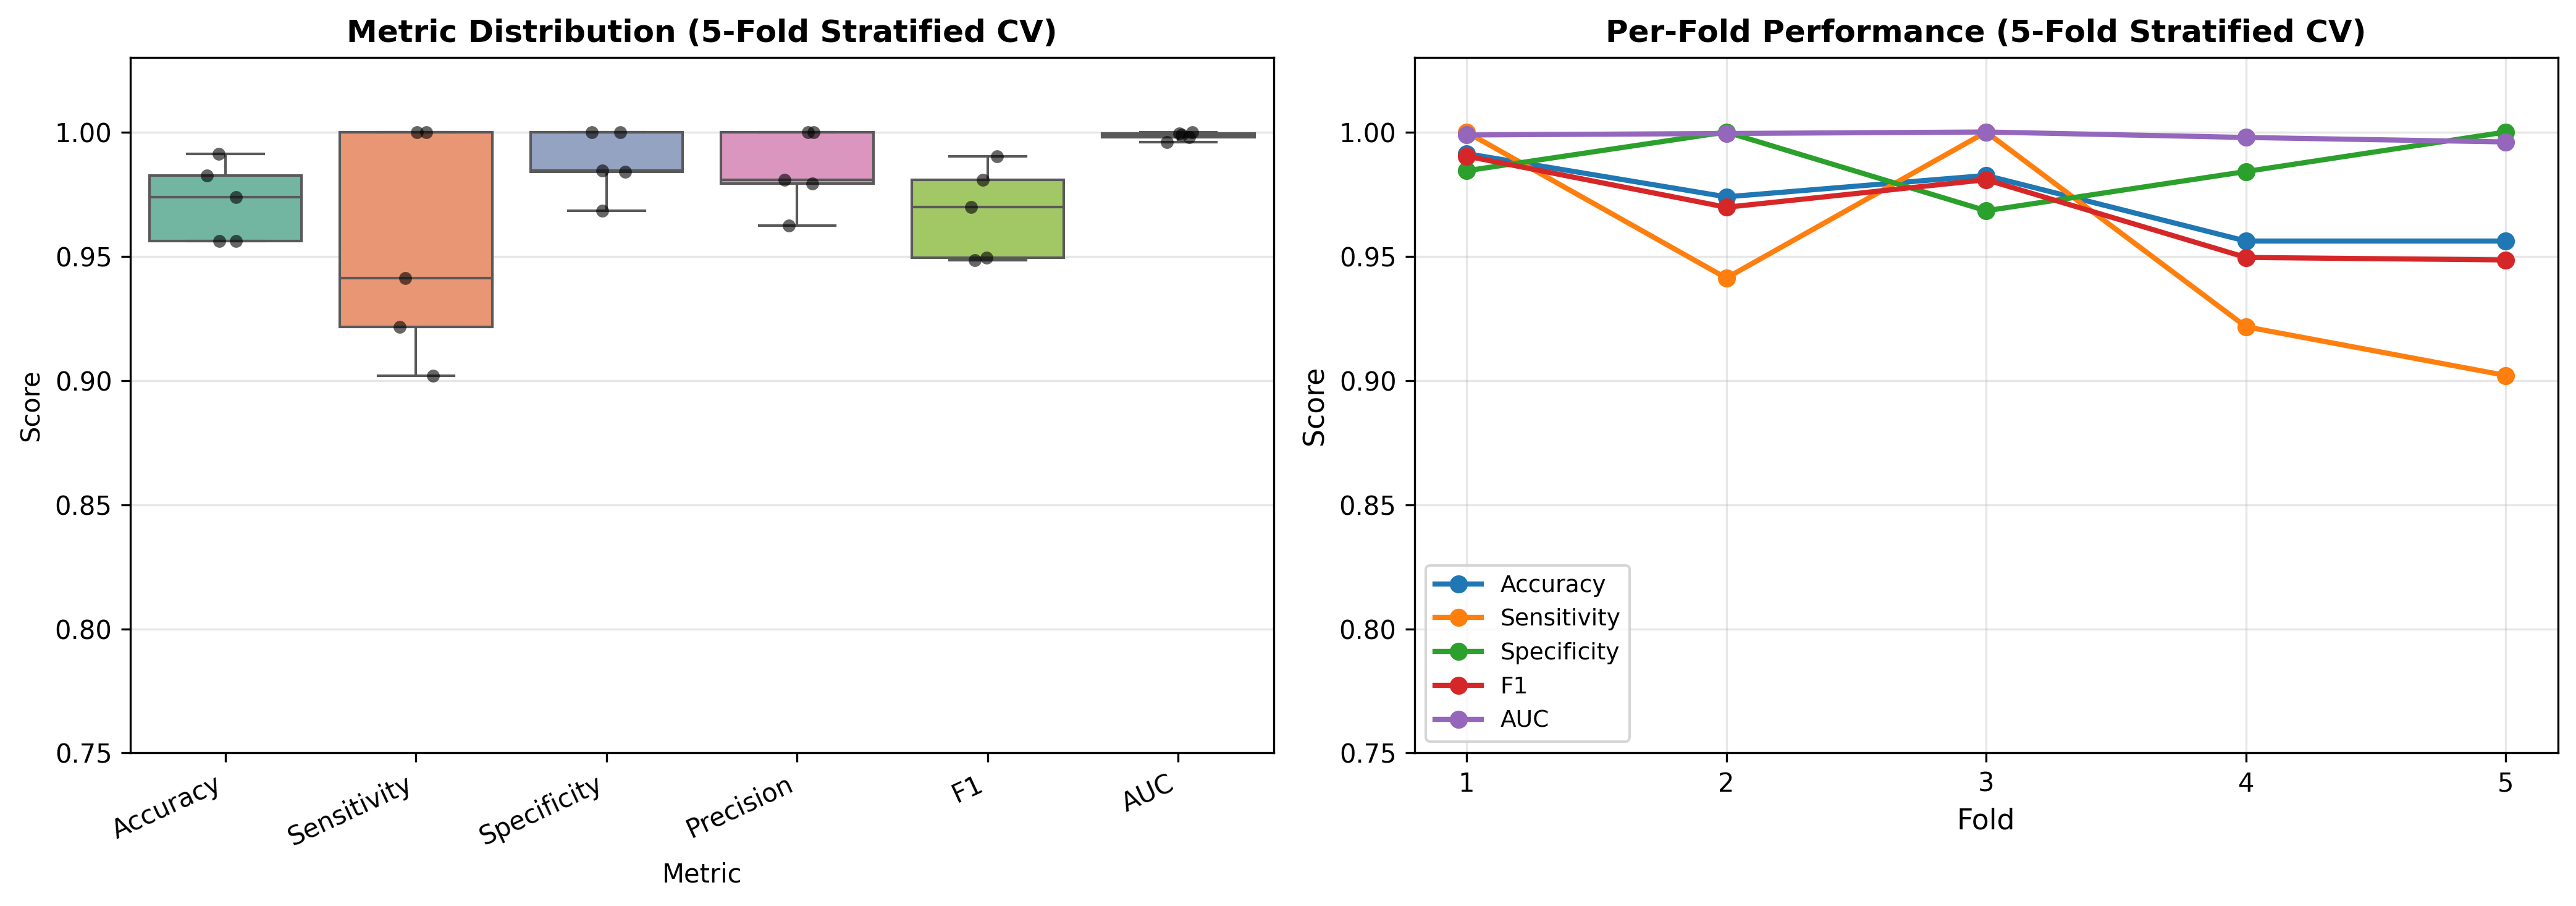
\includegraphics[width=0.98\textwidth]{figs/kfold_cv_metrics.png}
    \caption{Left: Boxplot distribution of classification metrics across the 5 stratified folds ($N=572$). Right: Per-fold metric trajectories.}
    \label{fig:kfold_cv}
\end{figure}

\begin{figure}[htbp]
    \centering
    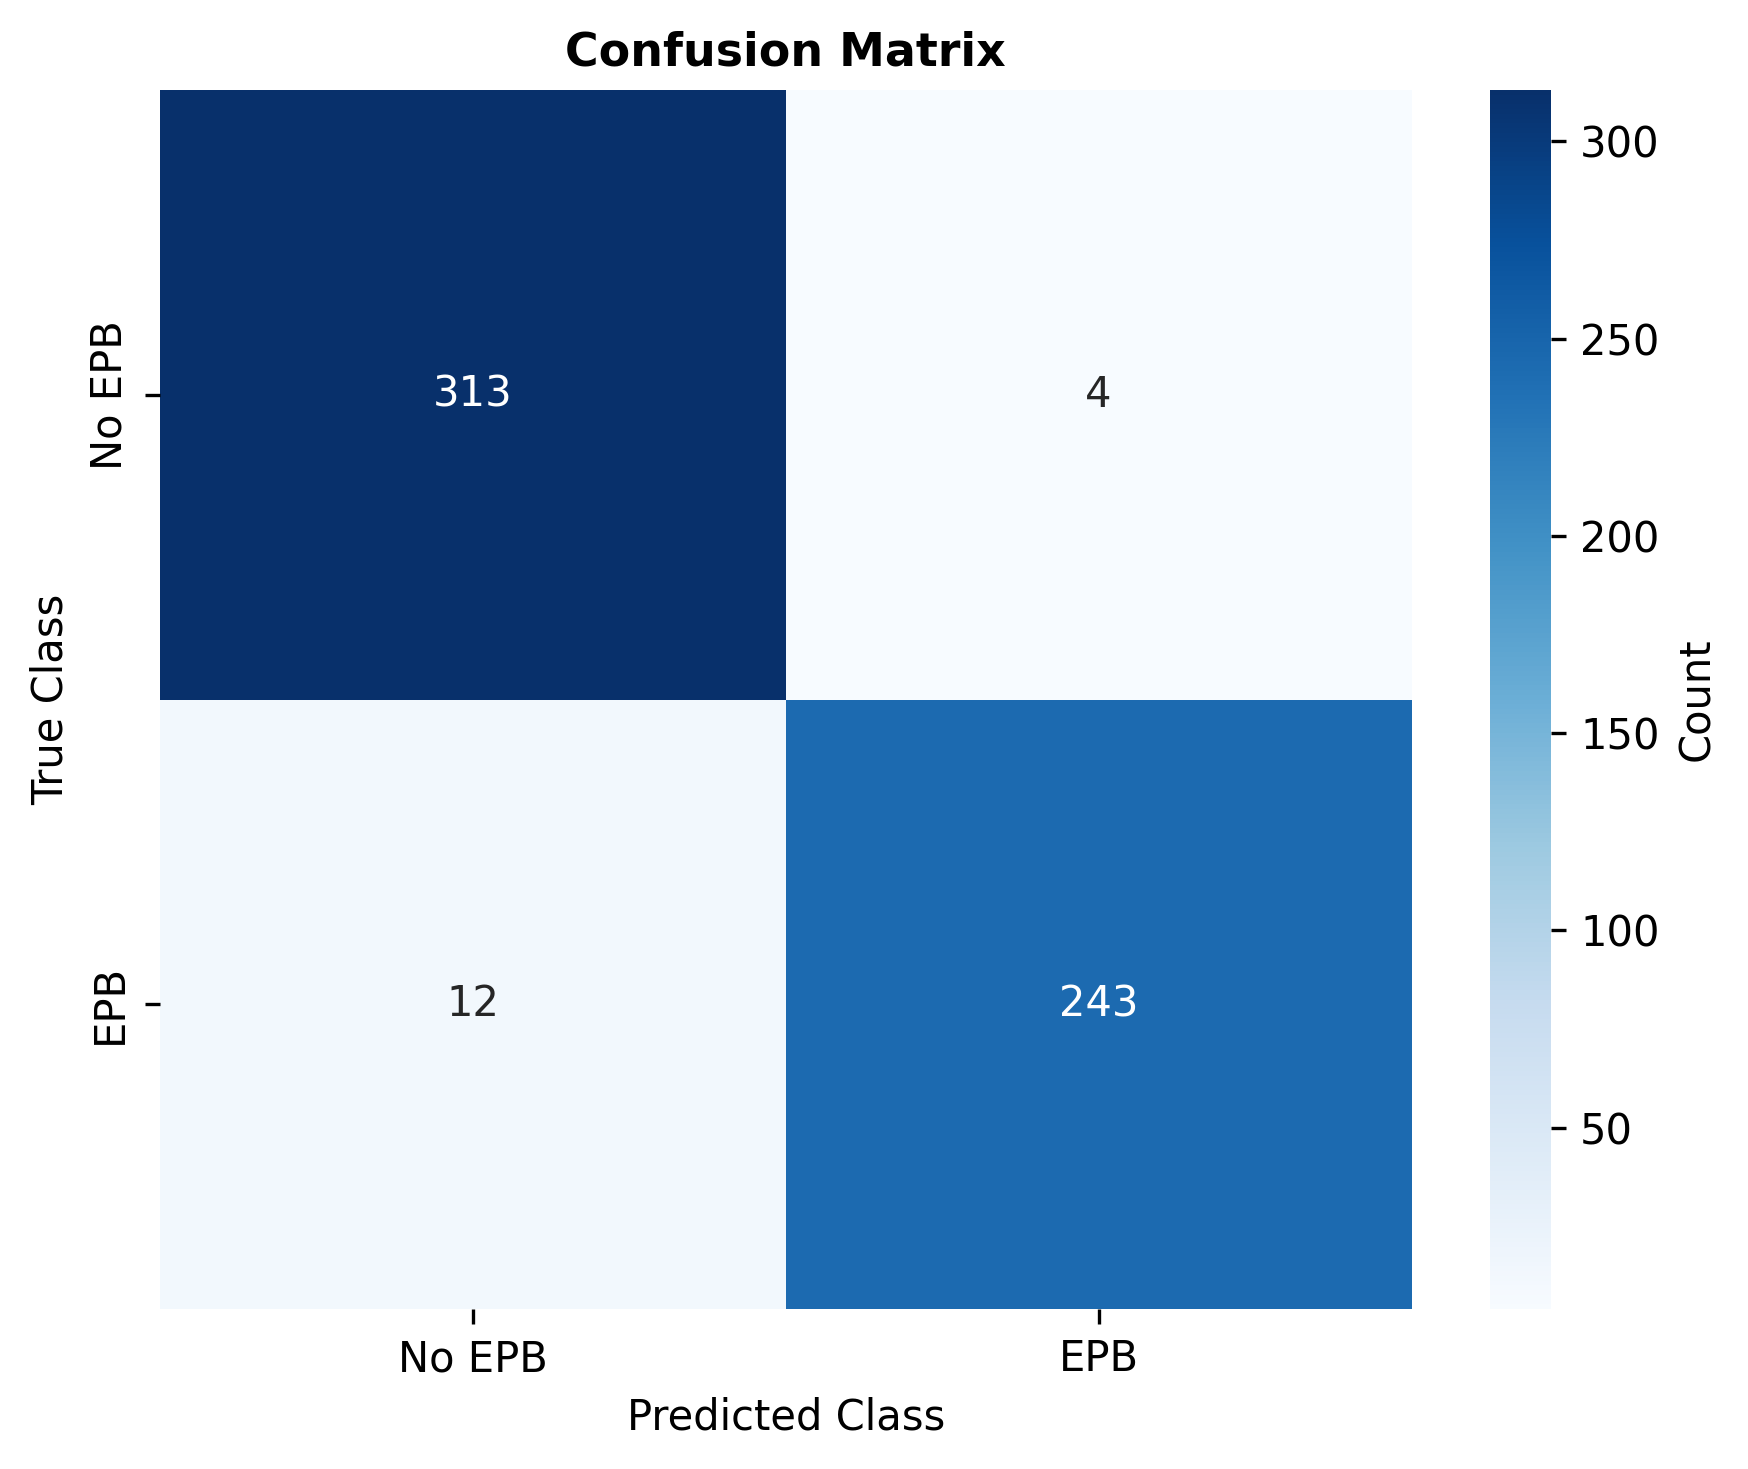
\includegraphics[width=0.52\textwidth]{figs/confusion_matrix.png}
    \caption{Out-of-fold confusion matrix aggregated across all $N=572$ labeled exposures ($313$ TN, $4$ FP, $12$ FN, $243$ TP).}
    \label{fig:confusion_matrix}
\end{figure}

\begin{figure}[htbp]
    \centering
    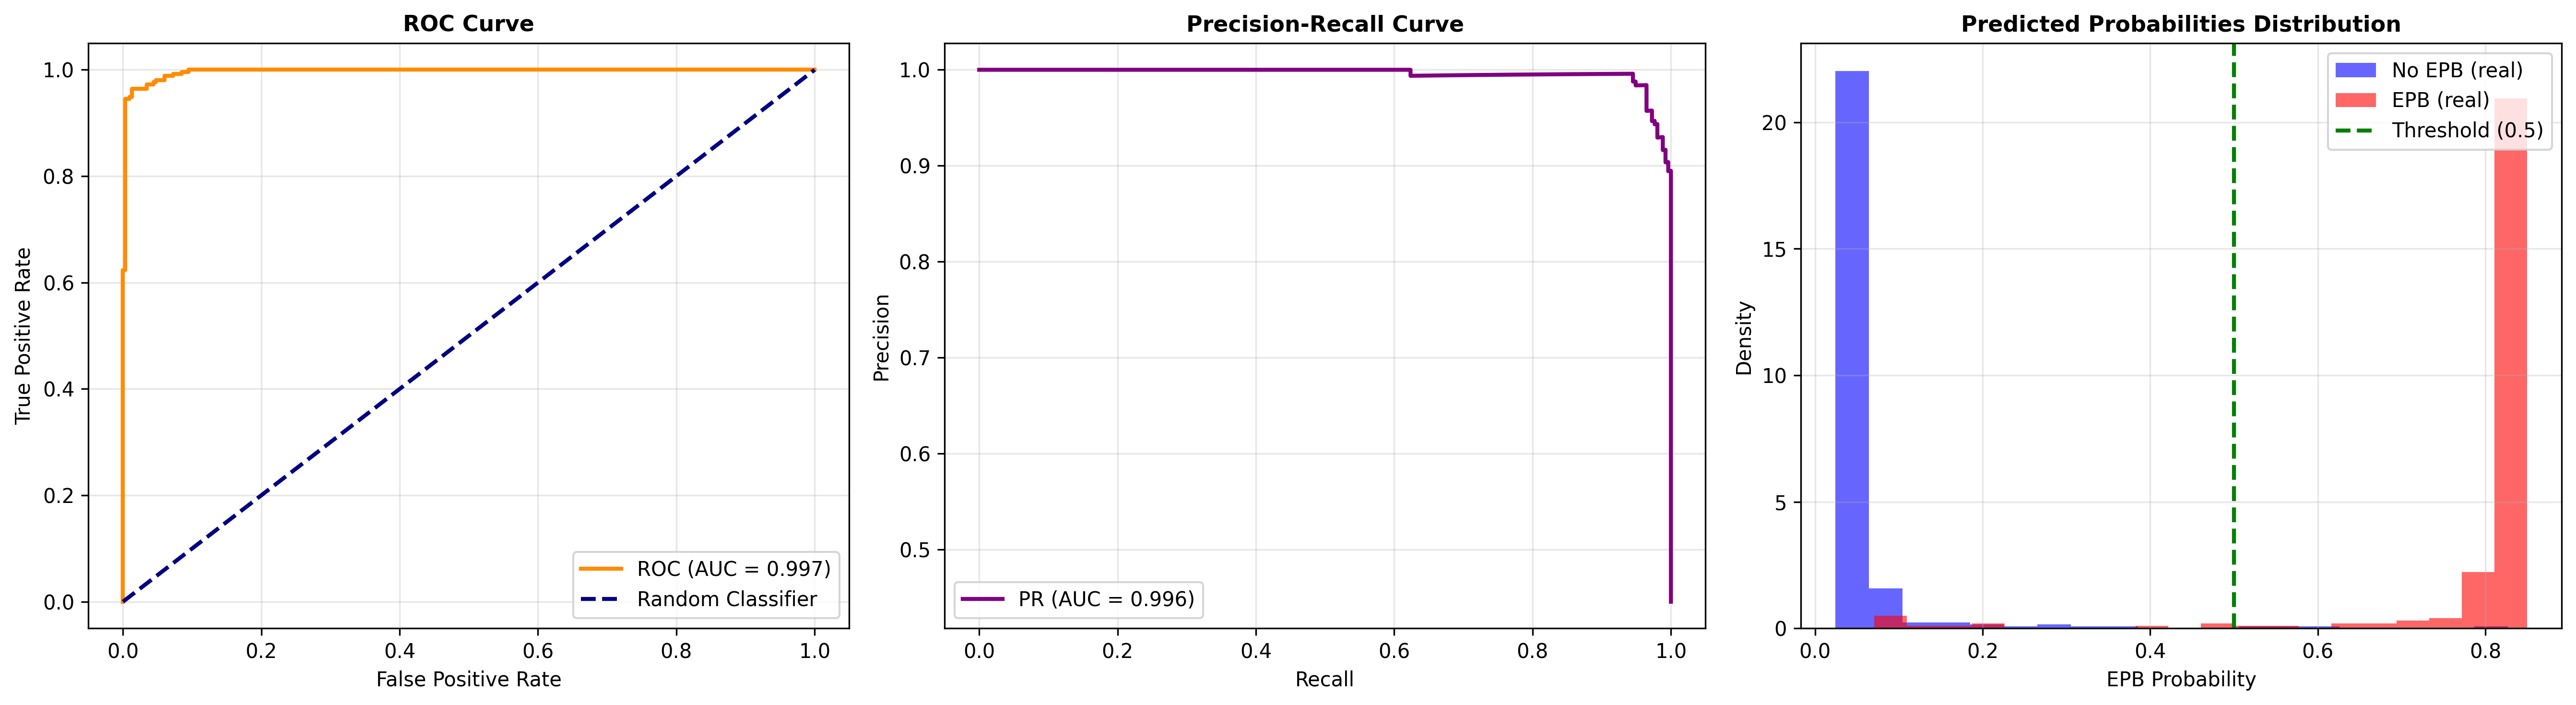
\includegraphics[width=0.98\textwidth]{figs/roc_pr_curves.png}
    \caption{Aggregated out-of-fold ROC curve (AUC $= 0.997$), Precision-Recall curve (AUC $= 0.996$), and predicted probability histogram across all $N=572$ labeled images.}
    \label{fig:roc_pr}
\end{figure}

When consecutive exposures from the same $30\text{-minute}$ window are forced into the same fold via 5-fold Temporal-Block Group Cross-Validation ($77$ non-overlapping blocks), the pipeline maintains $95.08\% \pm 5.72\%$ accuracy, $98.79\% \pm 2.71\%$ specificity, $94.24\% \pm 5.37\%$ F1-score, and $0.9969 \pm 0.0066$ ROC-AUC ($0.9978 \pm 0.0041$ PR-AUC). The higher fold-to-fold standard deviation in sensitivity ($90.88\% \pm 10.48\%$) reflects the fact that holding out entire half-hour active blocks removes specific depletion morphologies from training, yet the near-unity ROC-AUC ($0.9969$) shows that class ranking remains well separated without relying on frame-to-frame temporal leakage. Similarly, applying the circular FOV mask ($r = 0.44 \times 64$) to erase all corner timestamp and station-code text yields $95.80\% \pm 1.57\%$ 5-fold CV accuracy ($0.9976$ ROC-AUC) and $96.50\%$ holdout accuracy, confirming that the ensemble does not depend on burned-in text annotations.

\subsection{Baseline Comparison, Ablation Study, and Shortcut Analysis}

Table~\ref{tab:benchmark} and Figure~\ref{fig:benchmark} compare the proposed 2DPCA + Stacking Ensemble against flattened 1D classifiers, 1D-PCA baselines ($320$ components), individual 2DPCA base learners, an end-to-end 2D Convolutional Neural Network ($\text{AvgPool}_{2\times 2} \to \text{Conv2D}_{8,5\times 5} \to \text{MaxPool}_{2\times 2} \to \text{Conv2D}_{16,3\times 3} \to \text{MaxPool}_{2\times 2} \to \text{Dense}_{32} \to \text{Sigmoid}$, trained for $25$ epochs with Adam), and three ablations. To test whether high holdout scores reflect genuine ionospheric feature learning or station-level shortcut learning, every model was also trained exclusively on Cariri and Bom Jesus da Lapa ($n=530$) and evaluated zero-shot on the unseen Cachoeira Paulista observatory (ZS-CP, $n=42$).

\begin{table}[htbp]
\centering
\caption{Baseline and ablation comparison on the stratified holdout test set ($n=143$), zero-shot recall on the unseen Cachoeira Paulista observatory (ZS-CP, $n=42$), and single-frame CPU inference latency.}
\label{tab:benchmark}
\resizebox{\textwidth}{!}{%
\setlength{\tabcolsep}{4pt}
\begin{tabular}{lcccccccc}
\toprule
\textbf{Model / Ablation Configuration} & \textbf{Acc} & \textbf{Sens} & \textbf{Spec} & \textbf{Prec} & \textbf{F1} & \textbf{ROC-AUC} & \textbf{ZS-CP} & \textbf{ms/img} \\
\midrule
Flatten ($4096$) + Logistic Regression & 0.9790 & 0.9688 & 0.9873 & 0.9841 & 0.9764 & 0.9992 & 0.9762 & 0.050 \\
1D-PCA ($320$) + Logistic Regression & 0.9860 & 1.0000 & 0.9747 & 0.9697 & 0.9846 & 0.9994 & 0.6905 & 0.070 \\
1D-PCA ($320$) + SVM (RBF) & 0.9510 & 1.0000 & 0.9114 & 0.9014 & 0.9481 & 0.9921 & 1.0000 & 0.231 \\
Flatten ($4096$) + Random Forest & 0.9720 & 1.0000 & 0.9494 & 0.9412 & 0.9697 & 0.9996 & 0.5476 & 0.678 \\
2DPCA ($k=5$) + SVM (RBF) & 0.9650 & 0.9688 & 0.9620 & 0.9538 & 0.9612 & 0.9978 & 1.0000 & 0.087 \\
2DPCA ($k=5$) + Random Forest & 0.9371 & 0.9062 & 0.9620 & 0.9508 & 0.9280 & 0.9909 & 1.0000 & 0.749 \\
2DPCA ($k=5$) + XGBoost & 0.9510 & 0.9375 & 0.9620 & 0.9524 & 0.9449 & 0.9958 & 1.0000 & 0.027 \\
2D-CNN (ConvNet Baseline) & 0.9720 & 1.0000 & 0.9494 & 0.9412 & 0.9697 & 0.9974 & 1.0000 & 0.769 \\
\midrule
Ablation: No Physics Preprocessing & 0.9930 & 1.0000 & 0.9873 & 0.9846 & 0.9922 & 1.0000 & 0.0000 & 0.570 \\
Ablation: No SMOTE Balancing & 0.9650 & 0.9531 & 0.9747 & 0.9683 & 0.9606 & 0.9970 & 1.0000 & 0.621 \\
Ablation: Circular FOV Mask & 0.9650 & 0.9531 & 0.9747 & 0.9683 & 0.9606 & 0.9964 & 1.0000 & 0.456 \\
2DPCA + Stacking Ensemble (Proposed) & 0.9650 & 0.9531 & 0.9747 & 0.9683 & 0.9606 & 0.9974 & 1.0000 & 0.630 \\
\bottomrule
\end{tabular}%
}
\end{table}

\begin{figure}[htbp]
    \centering
    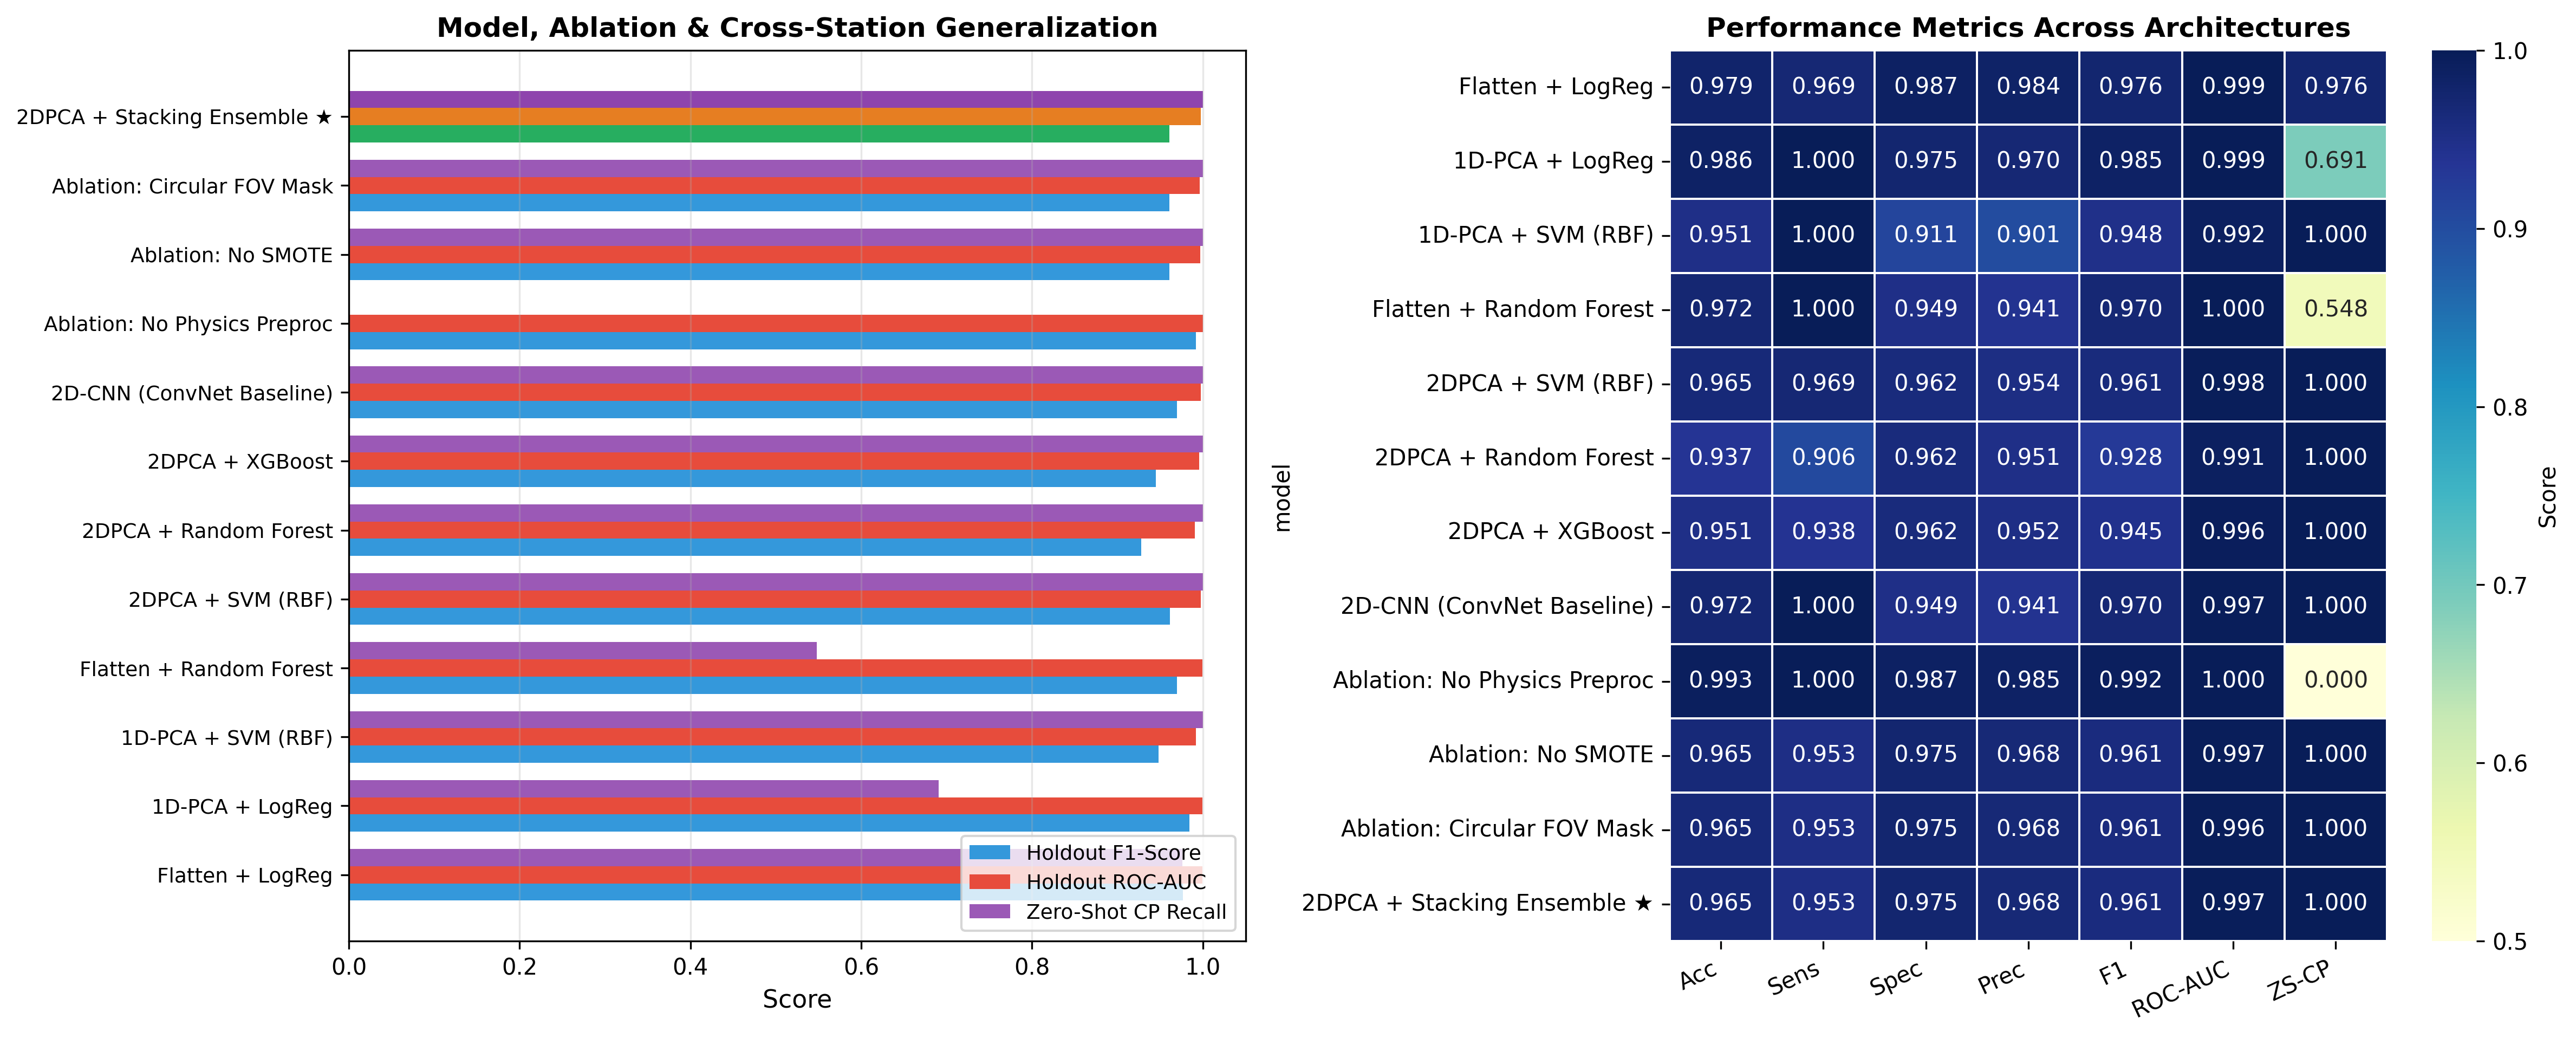
\includegraphics[width=0.98\textwidth]{figs/benchmark_baselines.png}
    \caption{Comparison of holdout F1-score, holdout ROC-AUC, and zero-shot Cachoeira Paulista recall (ZS-CP) across baselines, individual 2DPCA learners, 2D-CNN, and ablations.}
    \label{fig:benchmark}
\end{figure}

Table~\ref{tab:benchmark} reveals an important methodological finding. On the stratified holdout split alone, the raw-image ablation (No Physics Preprocessing) attains the highest apparent accuracy ($0.9930$), and flattened or 1D-PCA models reach $0.9720\text{--}0.9860$. However, when tested zero-shot on the unseen Cachoeira Paulista observatory (ZS-CP), the model without physics preprocessing fails completely, detecting $0/42$ EPB exposures ($0.0\%$ recall). Without Gaussian background subtraction and CLAHE, the classifier simply memorizes the raw camera exposure and background luminance levels that distinguish Bom Jesus da Lapa ($100\%$ No-EPB) from Cariri ($68.7\%$ EPB), which do not transfer to the brighter optical baseline of Cachoeira Paulista. Likewise, Flatten + Random Forest and 1D-PCA + Logistic Regression suffer sharp zero-shot drops to $54.76\%$ ($23/42$) and $69.05\%$ ($29/42$), respectively, because they weight localized pixel coordinates tied to individual station geometries.

In contrast, all models operating on preprocessed 2DPCA features achieve $100.0\%$ zero-shot recall ($42/42$) on Cachoeira Paulista. Within the 2DPCA group, the stacking ensemble combines the higher sensitivity of SVM ($96.88\%$) with the tree estimators to achieve higher specificity ($97.47\%$ vs. $96.20\%$ for single 2DPCA learners and $94.94\%$ for the 2D-CNN) at a sub-millisecond inference time of $0.630\text{ ms}$ per image. While omitting SMOTE leaves holdout accuracy unchanged ($0.9650$) due to the mild $1.24:1$ overall class ratio, retaining in-fold SMOTE improves zero-shot prediction confidence on unseen stations ($75.71\%$ vs. $68.50\%$ mean probability on CP) and guards against steeper local imbalances during grouped cross-validation.

\subsection{Lunar Glare, Cross-Station Transfer, and Stage 1 Cloud Screening}

Table~\ref{tab:hard_negatives} summarizes the three operational stress tests addressing lunar glare, cross-station transfer, and cloud contamination:
\begin{enumerate}
    \item Lunar glare stratification: Grouping the $572$ out-of-fold predictions by astronomical moon illumination shows that under low to moderate lunar illumination ($<50\%$, $n=475$), the pipeline reaches $97.47\%$ accuracy, $95.29\%$ sensitivity, and $100.0\%$ specificity ($220/220$). On the $97$ bright-moon exposures ($\ge 50\%$ illumination, up to $99.6\%$ full moon), where intense lunar glare saturates part of the dome, the classifier maintains $95.88\%$ specificity ($93/97$ correctly rejected as quiet sky), demonstrating that Gaussian background subtraction ($\sigma=10$) effectively removes smooth lunar illumination gradients.
    \item Cross-station performance: In 5-fold out-of-fold evaluation, accuracy is $94.84\%$ at Cariri ($n=310$, which contains both clear and partially cloudy transitions), $100.0\%$ at Bom Jesus da Lapa ($220/220$), and $100.0\%$ at Cachoeira Paulista ($42/42$). Under zero-shot holdout (trained on the $530$ images from CA and BJL), the ensemble detects all $42/42$ EPB frames at CP ($100.0\%$ recall, mean probability $75.71\%$).
    \item Cloud rejection on continuous nocturnal sequences: To evaluate how a clear-sky EPB classifier behaves when clouds roll in, Stage~2 was trained on the $510$ clear-sky labeled images (\texttt{cloudy} $= 0$) and tested on three full-night sequences in Table~\ref{tab:hard_negatives}. On the overcast sequence \texttt{CA\_20260624} ($62$ exposures, $0$ true EPBs), running Stage~2 alone triggers $61/62$ ($98.4\%$) false EPB alarms because CLAHE amplifies dark cloud edges into high-contrast bands. Enabling Stage~1 Sky Quality Control automatically flags $49/62$ frames ($79.0\%$) as overcast ($N_{\text{star}} < 4500$) and $7/62$ ($11.3\%$) as degraded visibility ($4500 \le N_{\text{star}} < 6500$), reducing false EPB triggers from $61$ to $13$ ($21.0\%$, a $78.7\%$ reduction) across all accepted frames, and down to $6$ ($9.7\%$, a $90.2\%$ reduction) when automated alerts are restricted to high-transparency \texttt{CLEAR} frames ($N_{\text{star}} \ge 6500$). On the clear quiet night \texttt{BJL\_20250722} ($230$ exposures), Stage~1 blocks $14$ twilight/haze frames ($6.1\%$) and eliminates all $3$ Stage~2 false triggers ($0.0\%$ false alarms, $100.0\%$ specificity). On the active EPB night \texttt{CA\_20251022} ($140$ exposures), Stage~1 flags only $4$ cloudy frames ($2.9\%$) while preserving $125$ valid EPB detections ($89.3\%$, with $122$ under high-visibility clear sky).
\end{enumerate}

\begin{table}[htbp]
\centering
\caption{Operational evaluation across lunar illumination regimes, observatory sites (including zero-shot transfer to CP), and continuous nocturnal sequences comparing Stage~2 alone (trained on clear skies, $n=510$) against the two-stage cascaded pipeline.}
\label{tab:hard_negatives}
\resizebox{\textwidth}{!}{%
\setlength{\tabcolsep}{4.5pt}
\begin{tabular}{llcccc}
\toprule
\textbf{Evaluation Scenario} & \textbf{Protocol / Mode} & \textbf{Frames} & \textbf{QC Flagged} & \textbf{Metric / Result} \\
\midrule
Low/Moderate Moon ($<50\%$) & 5-Fold OOF & 475 & -- & Acc: $97.47\%$ / Spec: $100.0\%$ ($220/220$) \\
Bright Lunar Glare ($\ge 50\%$) & 5-Fold OOF (Hard Neg.) & 97 & -- & Specificity: $95.88\%$ ($93/97$) \\
\midrule
São João do Cariri (CA) & 5-Fold OOF & 310 & -- & Accuracy: $94.84\%$ \\
Bom Jesus da Lapa (BJL) & 5-Fold OOF & 220 & -- & Specificity: $100.0\%$ ($220/220$) \\
Cachoeira Paulista (CP) & Zero-Shot (Train: CA+BJL) & 42 & -- & Recall: $100.0\%$ ($42/42$) \\
\midrule
\texttt{BJL\_20250722} (Clear Quiet) & Stage 2 Only vs. Cascaded & 230 & $14$ ($6.1\%$) & FP: $3 \to 0$ ($100.0\%$ Spec.) \\
\texttt{CA\_20260624} (Overcast Sky) & Stage 2 Only vs. Cascaded & 62 & $49$ ($79.0\%$) & FP: $61 \to 13$ ($6$ Clear, $-78.7\%$ / $-90.2\%$) \\
\texttt{CA\_20251022} (Active EPB) & Stage 2 Only vs. Cascaded & 140 & $4$ ($2.9\%$) & Valid EPB: $125$ ($89.3\%$) \\
\bottomrule
\end{tabular}%
}
\end{table}

\subsection{Supervised SHAP Attribution and Nocturnal Time Series}

Figures~\ref{fig:shap_without} and~\ref{fig:shap_with} display the supervised pixel-space SHAP attribution maps ($\boldsymbol{\Phi}_{\text{pixel}} = \boldsymbol{\Phi}_{\text{feat}}\mathbf{W}^\top$) for representative quiet-sky and active EPB exposures. Because each feature \texttt{PC\_Row\_$r$\_Comp\_$c$} corresponds to horizontal row $r$ projected onto eigenvector $c$, back-projecting the tree SHAP values through $\mathbf{W}^\top$ localizes the exact rows and columns driving the ensemble output.

\begin{figure}[htbp]
    \centering
    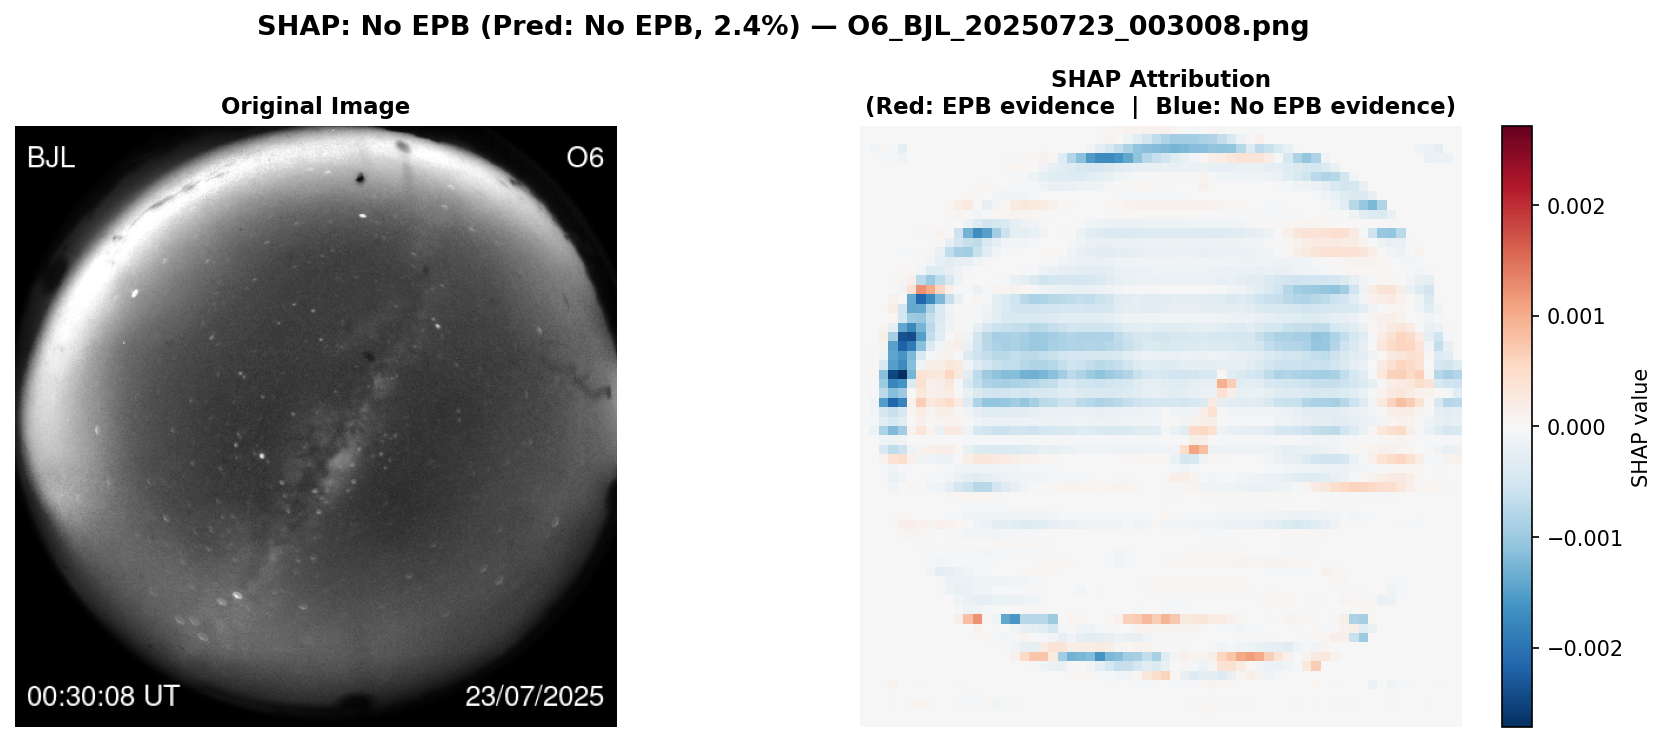
\includegraphics[width=0.98\textwidth]{figs/shap_analysis_without.png}
    \caption{Pixel-space SHAP attribution for a quiet-sky exposure from Bom Jesus da Lapa (True: No EPB, Predicted: No EPB, $0.4\%$). Blue regions denote negative attributions that reduce EPB probability.}
    \label{fig:shap_without}
\end{figure}

\begin{figure}[htbp]
    \centering
    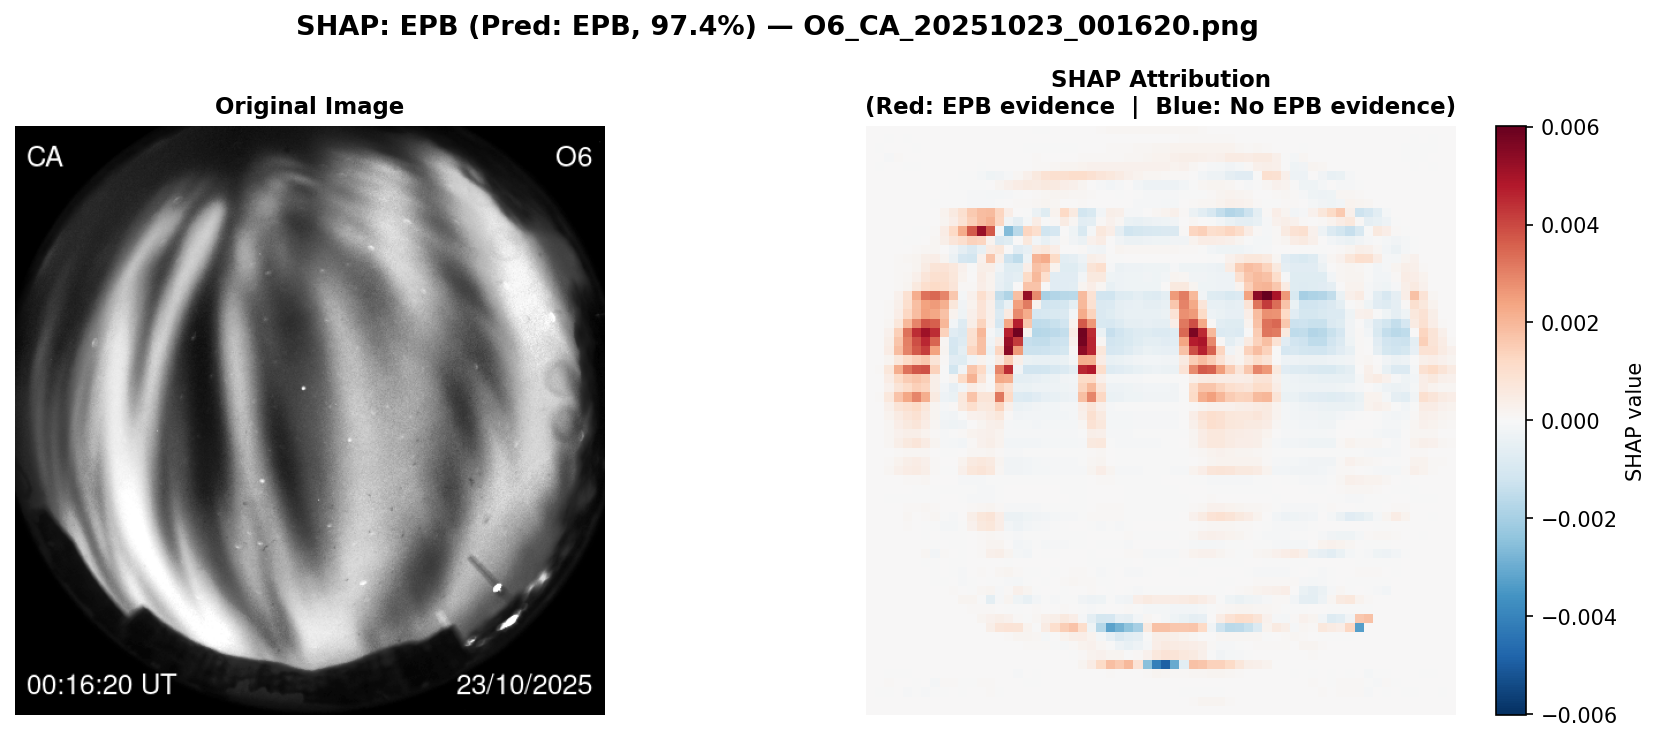
\includegraphics[width=0.98\textwidth]{figs/shap_analysis_with.png}
    \caption{Pixel-space SHAP attribution for an active EPB exposure from Cariri (True: EPB, Predicted: EPB, $99.2\%$). Red bands mark positive attributions aligned with the plasma depletion channels.}
    \label{fig:shap_with}
\end{figure}

In the quiet exposure (Figure~\ref{fig:shap_without}), negative (blue) SHAP values dominate the central dome, suppressing the predicted EPB probability to $0.4\%$. In the active exposure (Figure~\ref{fig:shap_with}), positive (red) SHAP attributions align with the dark North-South depletion bands across the central sky dome ($99.2\%$ predicted probability), while the four image corners containing text overlays receive near-zero attribution.

\begin{figure}[htbp]
    \centering
    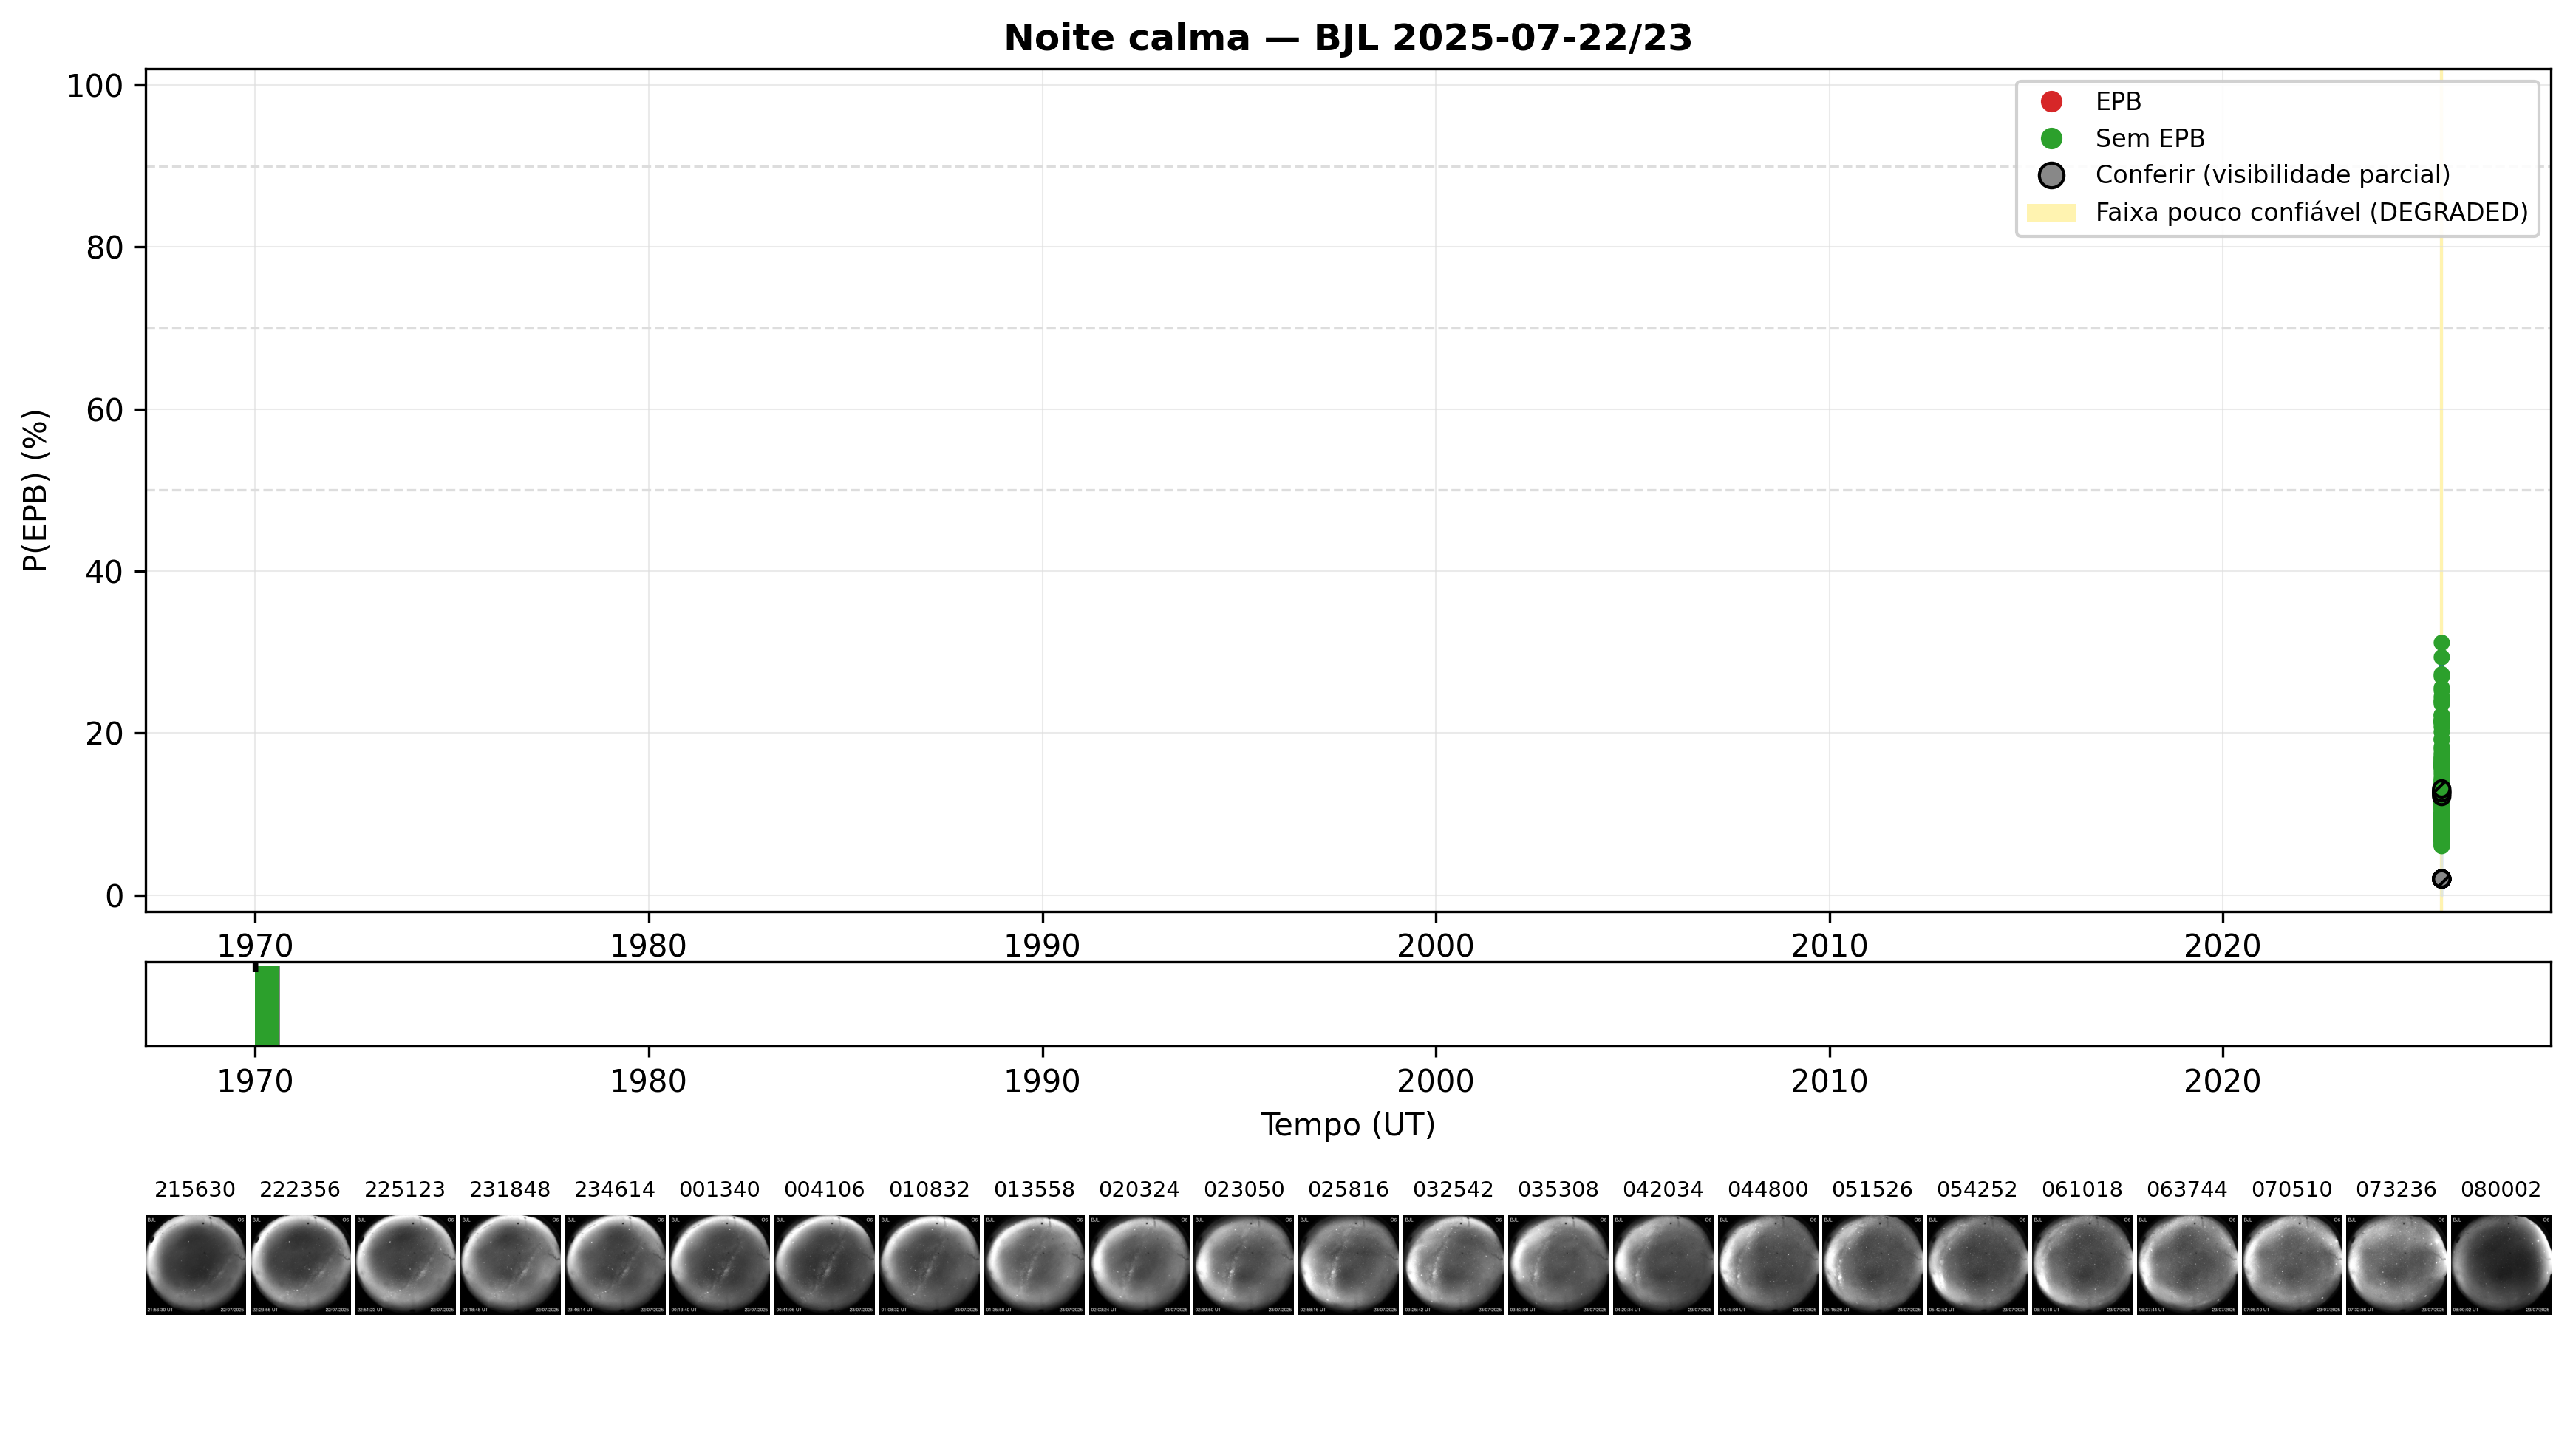
\includegraphics[width=0.98\textwidth]{figs/temporal_without_epb.png}
    \caption{Nocturnal time series on a clear quiet night at Bom Jesus da Lapa (\texttt{BJL\_20250722}, $230$ exposures). Predicted EPB probabilities remain near $0.4\%$ all night ($0$ false alarms).}
    \label{fig:temporal_without}
\end{figure}

\begin{figure}[htbp]
    \centering
    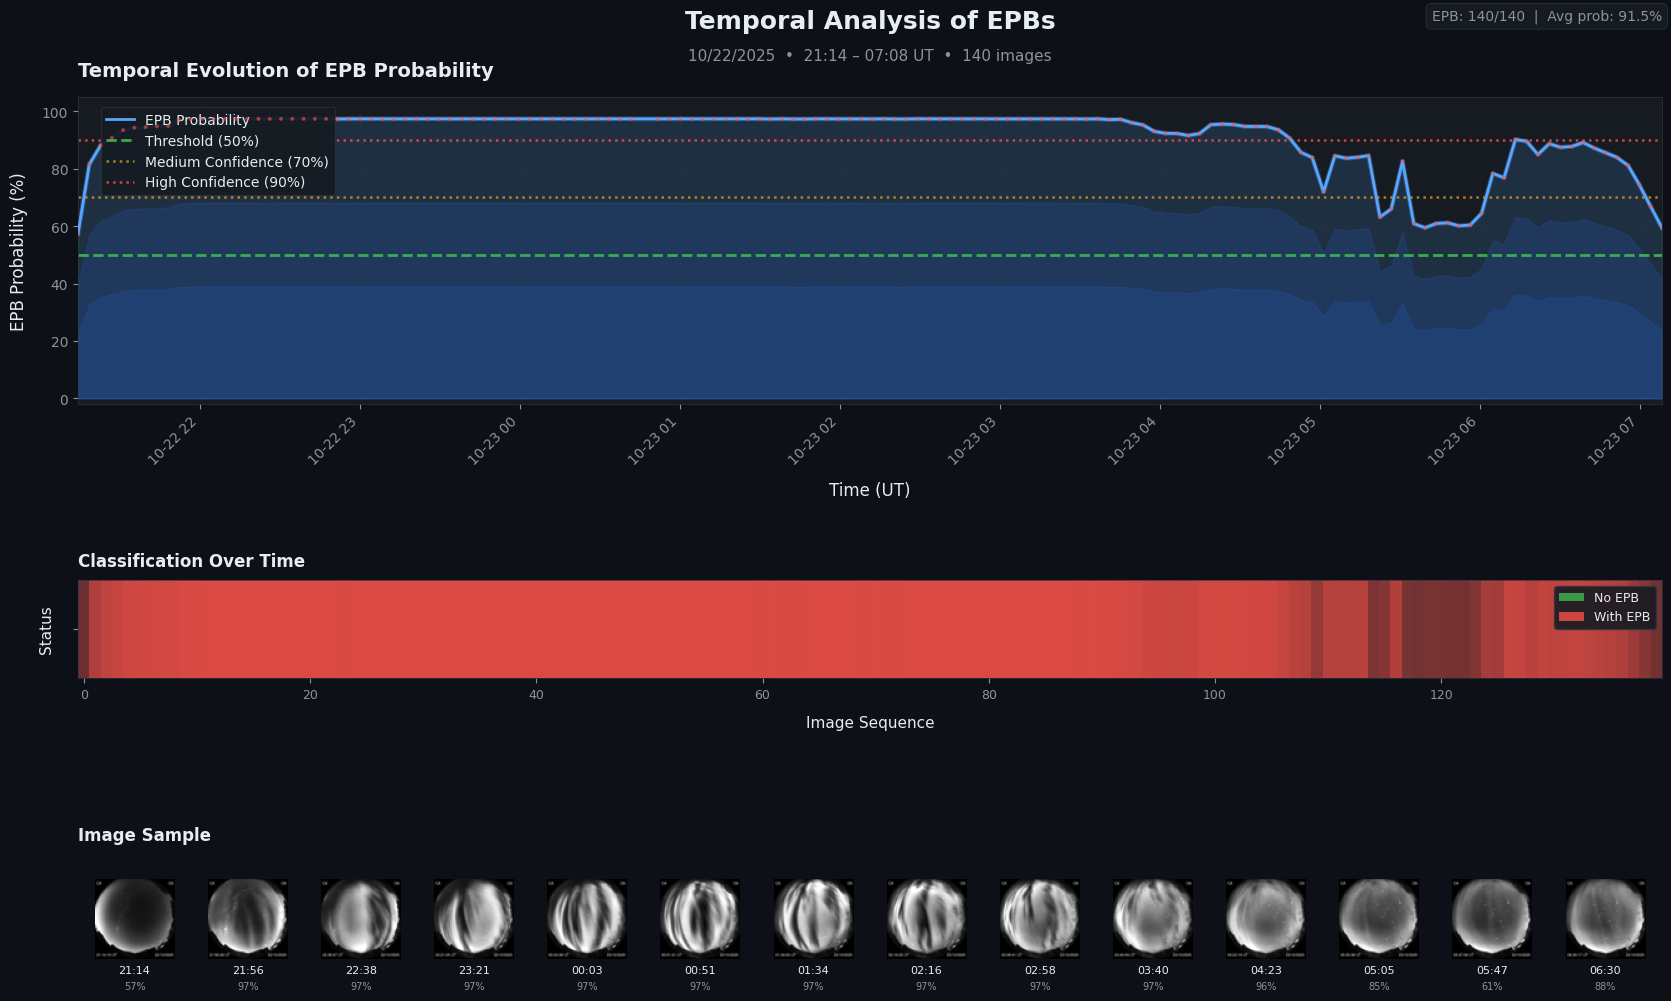
\includegraphics[width=0.98\textwidth]{figs/temporal_with_epb.png}
    \caption{Nocturnal time series on an active EPB night at Cariri (\texttt{CA\_20251022}, $140$ exposures), capturing bubble onset after $21{:}18\text{ UT}$, sustained zenith passage ($138/140$ frames), and pre-dawn decay.}
    \label{fig:temporal_with}
\end{figure}

\begin{figure}[htbp]
    \centering
    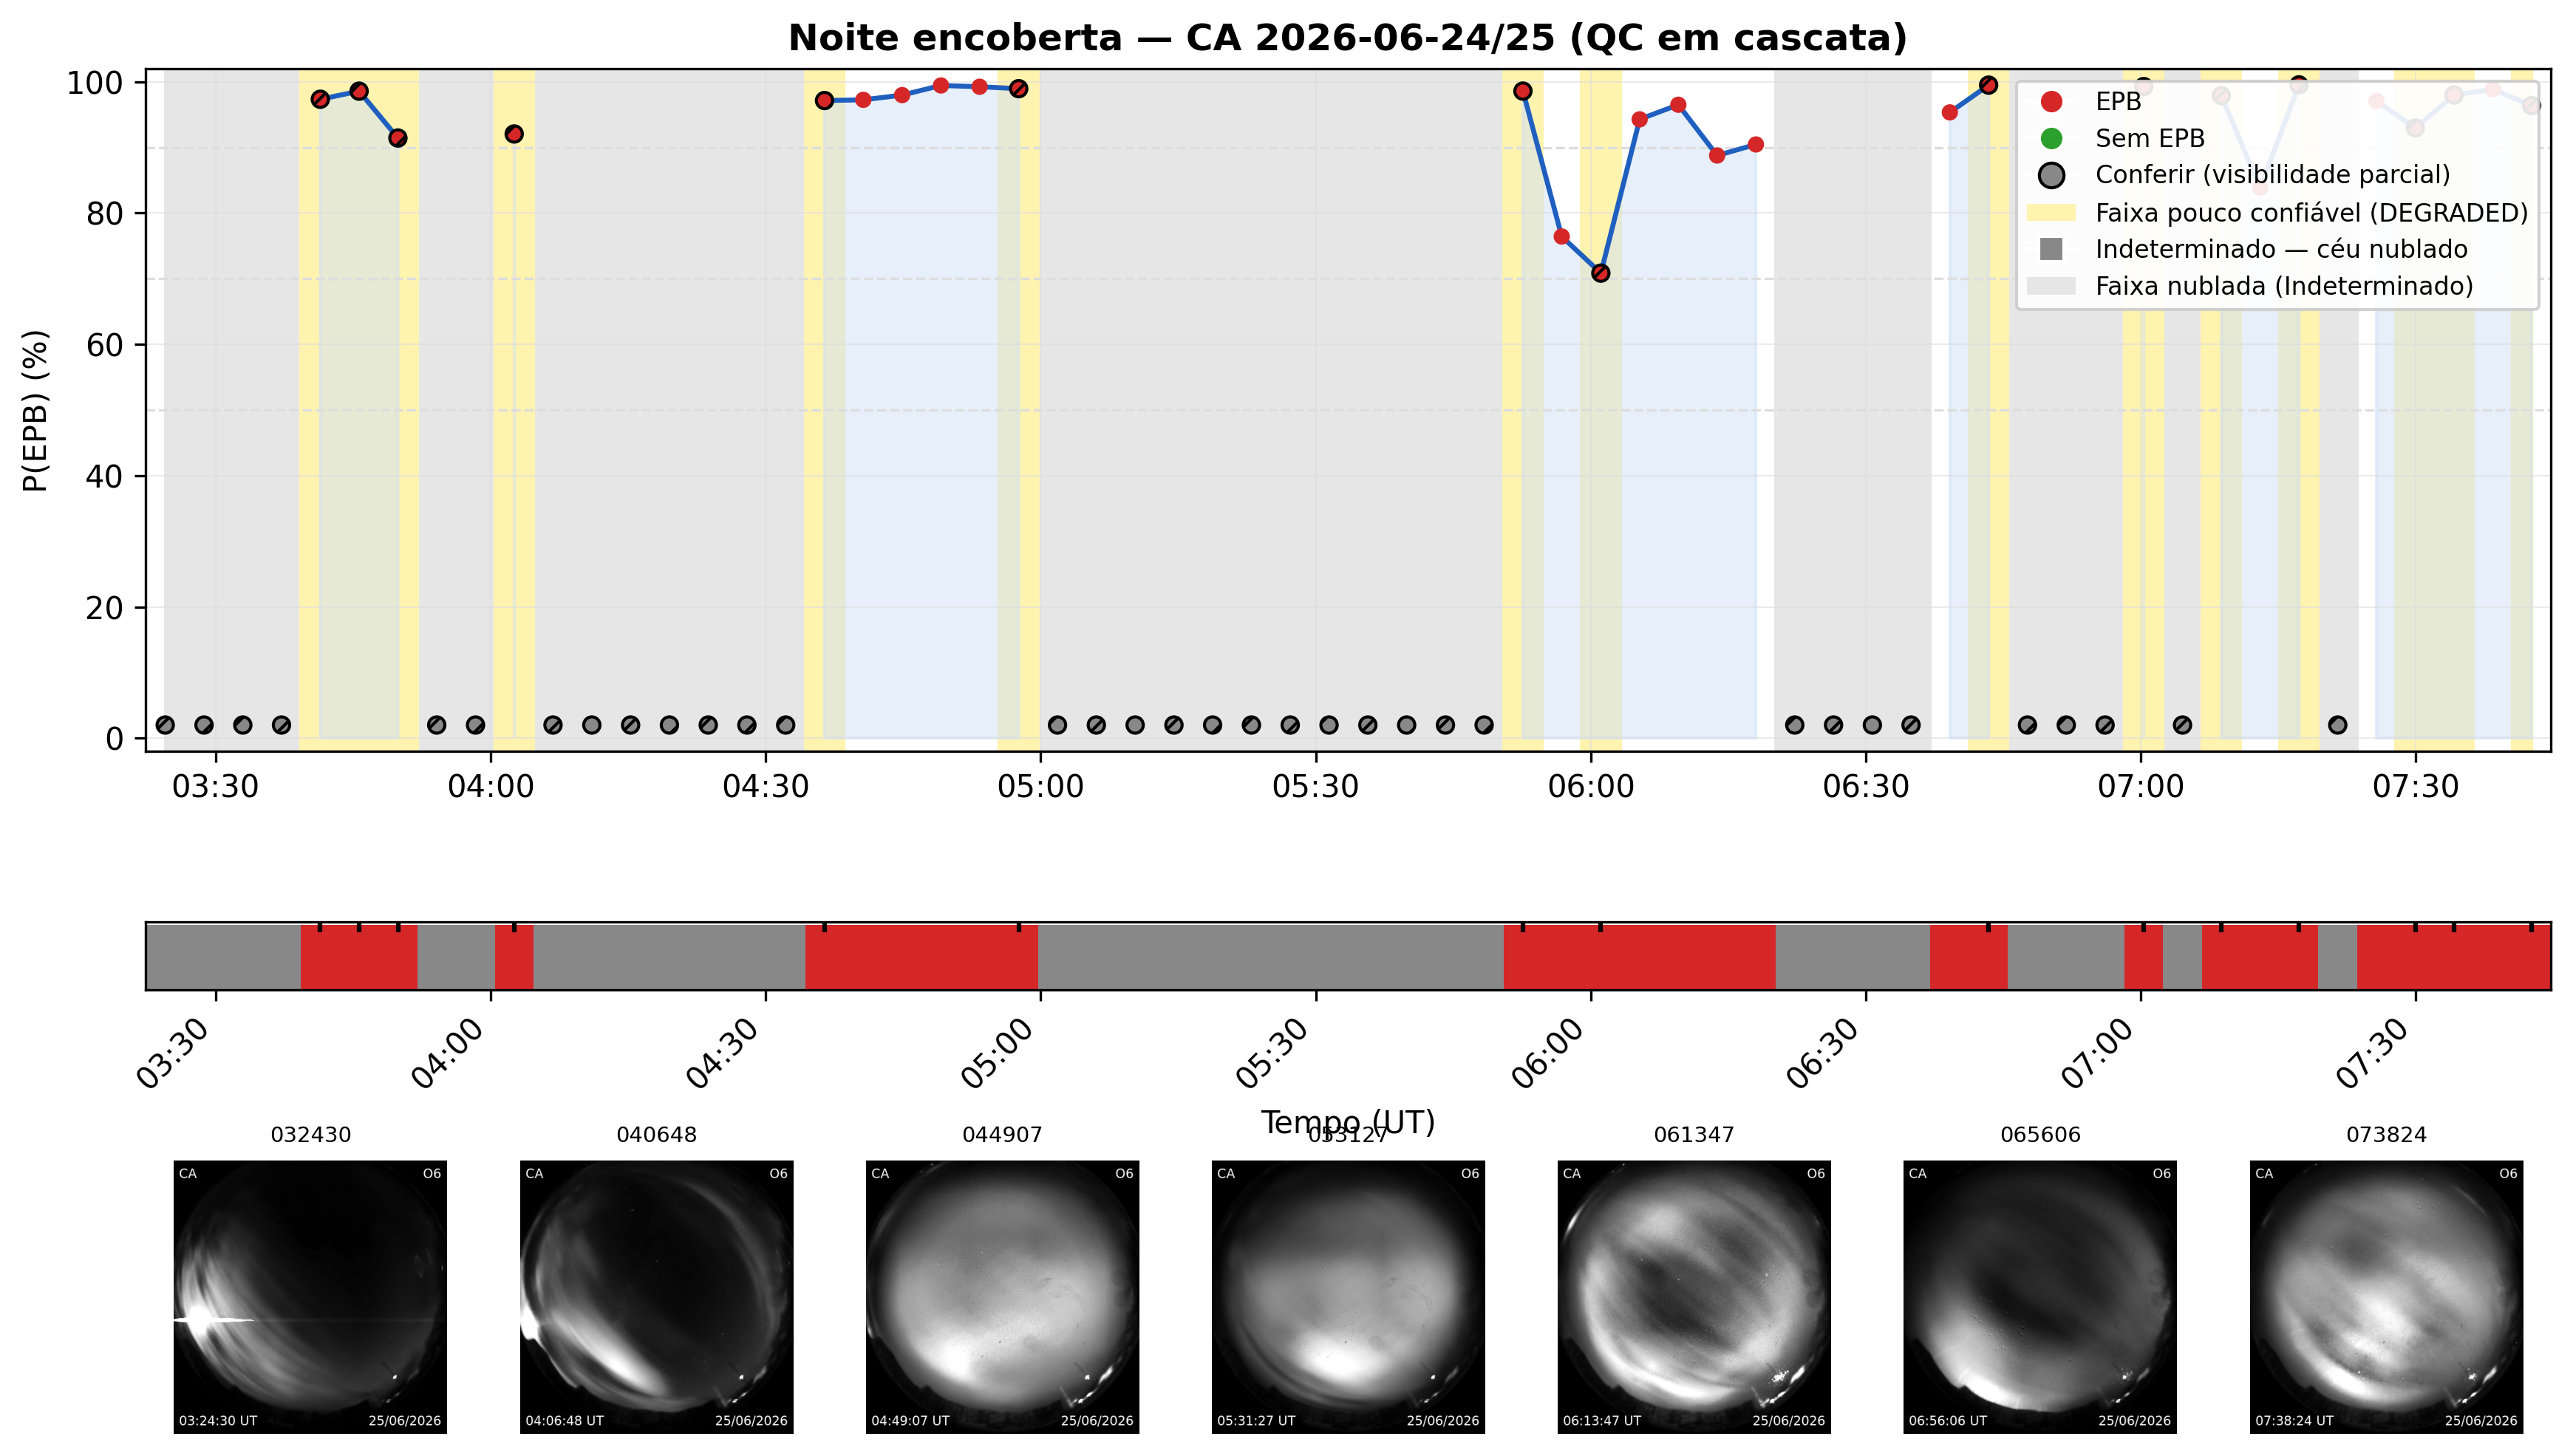
\includegraphics[width=0.98\textwidth]{figs/temporal_cloudy_qc.png}
    \caption{Cascaded nocturnal monitoring on an overcast night at Cariri (\texttt{CA\_20260624}, $62$ exposures). Stage~1 Sky QC (gray status intervals) flags $49/62$ frames ($79.0\%$) as cloudy.}
    \label{fig:temporal_cloudy}
\end{figure}

Figures~\ref{fig:temporal_without}--\ref{fig:temporal_cloudy} illustrate continuous full-night monitoring using the deployed model (\texttt{v4.0}). Across all $230$ exposures of the quiet night \texttt{BJL\_20250722} (Figure~\ref{fig:temporal_without}), the predicted EPB probability remains flat around $0.4\%$ with zero false alarms. During the active night \texttt{CA\_20251022} ($140$ exposures, Figure~\ref{fig:temporal_with}), the probability rises above the threshold at $21{:}18\text{ UT}$ ($63.8\%$) and reaches $99\%$ as fully developed plasma bubbles cross the zenith, remains elevated through the night ($92.0\%$ mean probability across $138/140$ frames), and drops to $2.1\%$ as the depletions dissipate near dawn ($07{:}08\text{ UT}$). On the overcast night \texttt{CA\_20260624} ($62$ exposures, Figure~\ref{fig:temporal_cloudy}), Stage~1 Sky QC automatically masks $49/62$ frames ($79.0\%$) during prolonged cloud cover, leaving only brief partial clearings for Stage~2 evaluation.
